% !TEX root = ../2021_microservices_wileytemplate.tex

\section{Study Design}\label{sec:study-design}

We conducted a systematic literature review (SLR) conforming to the guidelines presented by Kitchenham and Charters~\cite{Kitchenham2007}. A systematic literature review (SLR) is a method of reviewing data and results from research about a particular question in a standardized systematic way~\cite{Sebastian2018}. According to Garousi et al.~\cite{Garousi2016}, it is important to complement scientific papers in an systematic literature review by also analyzing grey literature. Therefore, we decided to adapt our systematic literature review protocol to include grey references.


In this section, we describe the designed protocol for our systematic literature review which was enhanced with grey literature. We divided our protocol for the systematic literature review into the following steps: (1) Preparation, (2) Research questions, (3) Search procedure, (4) Selection criteria, (5) Grey literature, (6) Data extraction, and (7) Data synthesis.

\subsection{Preparation}

This step is called background by Kitchenham and Charters~\cite{Kitchenham2007}. After we defined the protocol, we started by reading papers about microservices to understand the current scope of microservices research. 

The first papers we study were a systematic literature review~\cite{Ghani2019} and systematic mapping studies~\cite{Claus2016, Francesco2019} since both types provide an overview of the state of the art on microservices. Then, we performed a backwards snowballing procedure to gather more references for this initial knowledge on microservices research~\cite{Shady2020, Michael2018, Toledo2019, Dragoni2017, Kevin2015, Larrucea2018, Osses2019, Meshenberg2016, Matt2016, Soldani2018, Olaf2016}.

Based on the studied references, we developed the rationale for this study (Sections I and II). Moreover, with an understanding of the research state-of-the-art, we were prepared to elaborate the research questions we aimed to investigate. 

\subsection{Research Questions}

The leading goal of this research is to analyze the possible challenges in adopting microservices. Moreover, we have also deemed it important to cover the technologies used in implementing microservices and solving such challenges. Therefore, we elaborated the following research questions to guide our systematic literature review:

\begin{itemize}
  \item RQ\#1: What are the main challenges when adopting microservices?
  \item RQ\#2: What are the main technologies used for implementing microservices?
\end{itemize}


\subsection{Search Procedure}

This step describes the search procedure we followed to acquire scientific references. 
We planned our procedure to search for microservices papers that would discuss challenges and technologies (i.e., tackle our research questions) but without biasing the search results. 
We performed a manual search using google scholar as the search engine. 
We chose google scholar because it combines results from multiple digital libraries. 
Moreover, citations and patents were excluded from the search.

We developed a strategy to choose the appropriate search string for our research. Two authors brainstormed and propose candidate strings. For each candidate string, we analyzed if the top results seem relevant for our research. We also needed a string that would not give too many results for the authors to handle manually. Therefore, the total number of results was also a factor in choosing the string. Moreover, we did not want the search string to be biased. After one week of analyzing candidate strings, we settled on the following: \texttt{microservices "architecture style" design}. The chosen string produces 471 references at the time we collected its results (2020-11-12). 
%Figure~\ref{fig:total-papers-per-year} shows the search results divided per year.

%\begin{figure}[h]
%	\centering
%	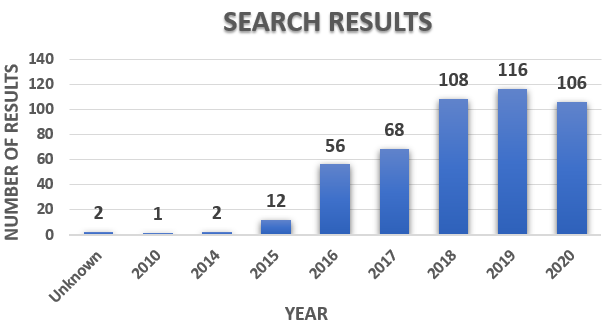
\includegraphics[width=0.5\linewidth]{images/yearvsarticles.png}
%	\caption{Search results per year before applying the selection criteria.}
%	\label{fig:total-papers-per-year}
%\end{figure}	 


\subsection{Selection Criteria}

Selection criteria determine which studies to include or exclude from a systematic literature review. 
Since the search provided a good amount of results, we focused on defining rejection criteria to exclude irrelevant results.
Our selection criteria are detailed as follows:
%Table~\ref{tab:selection-criteria} summarizes our selection criteria which we detail as follows:

%\begin{table}[h]
%\centering
%\caption{Selection Criteria}
%\label{tab:selection-criteria}
%\begin{tabular}{|l|p{5cm}|}
%\hline
%	& \\
%	& R1: Duplicate papers \\
%  	& R2: Not written in English \\
%   	& R3: Not peer-reviewed \\
%Exclusion Criteria    
%	& R4: Published before 2017 \\
%   	& R5: Select Extended versions \\
%   	& R6: Unrelated based on title \\
%   	& R7: Unrelated based on abstract  \\
%   	& \\
%\hline
%\end{tabular}
%\end{table}


\begin{itemize}
   \item \textbf{R1: Duplicated papers.} The search engine we used acquires papers from multiple libraries. Therefore, the results can contain the same paper more than once but from different sources. Then, we reject all duplicated instances of a paper that is already in our study.
   \item \textbf{R2: Not written in English.} A paper can have an English abstract and keywords even though the paper content is written in another language. The search engine may still present such papers based on their abstracts.
  \item \textbf{R3: Not peer-reviewed.} Some digital libraries allow users to post papers that were not peer-reviewed. Since the selection criteria are to choose scientific papers,  peer-review is very important to maintain academic integrity. We rejected all papers that were not peer-reviewed.
   \item \textbf{R4: Publication from 2017 to 2020.} 
We exclude papers published before 2017. We wanted this study to focus on the most recent studies on microservices.
  \item \textbf{R5: Multiple versions.} When a paper has multiple versions of itself, we reject the previous versions and keep only the most current one. For example, if a paper published on a conference is later extended to a journal paper, we would reject the conference version and keep the journal as it is the most current.
  \item \textbf{R6: Unrelated based on title.} For this criterion, we read the title of the paper to assess if it was indeed a relevant study to answer our research questions. The titles deemed unrelated were excluded.
  \item \textbf{R7: Unrelated based on abstract.} For this criterion, we read the abstract of the paper to verify if it would help to answer our research questions. The abstracts that were not related to our research were rejected.  
\end{itemize}


We apply the selection criteria in the same order as shown, i.e., we apply R1 first then followed by R2, and so forth.
From the described selection criteria, only the last two (R6 and R7) are subjective. To mitigate the subjectiveness of such criteria, we had two persons (the first and second authors) working separately to review them. In case of disagreement, the paper would be included in study. Therefore, we only rejected papers if both persons marked it as unrelated.

As we previously described, the search returned a total of 471 results. After applying our selection criteria, we obtained 60 studies (i.e., 311 papers were rejected). Figure~\ref{fig:selection-criteria} shows the number of papers rejected by each criterion, and 'A' marks the total of accepted papers after the rejection criteria were applied.

%The selection criteria are used to determine which studies could be included and excluded as shown in table 1. We analyze the data on the specific questions and which are most relevant to the answer the questions. Below table 1 shows the inclusion, exclusion criteria as determined from the research questions generated after the selection of the primary study. A study will be disqualified if it meets any of the following exclusion criteria. The study selection criterion has two major phases. In the first phase, the study inclusion/exclusion steps were applied as shown from i1 to i4 and R1 to R5. In the second phase, the study screening criterion was applied to the Title and Abstract. In both of the phases, the focus of the study is on microservices, and the existence of empirical work was ensured. As a result of the first screening phase (Title and Abstract screening), we obtained 471 studies as shown in figure 1. These 471 studies were screened for full-text inclusion/exclusion in the second phase. After applying inclusion/exclusion criteria to the full text we obtained 60 studies. In figure 2, the Exclusion criteria stepwise study screening process count is shown along with the number of studies excluded after each screening step. 

\begin{figure}[h]
	\centering
	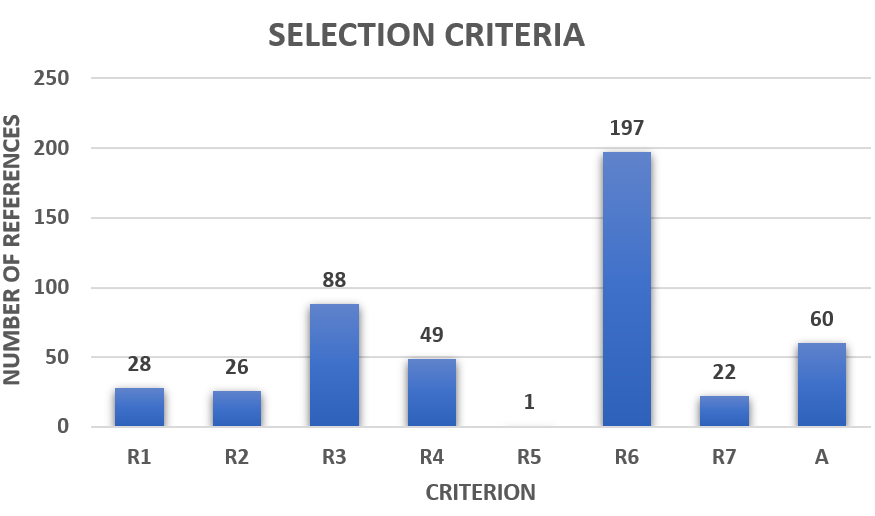
\includegraphics[width=0.5\linewidth]{images/exclusion.png}
	\caption{Selection criteria showing the number of scientific references rejected by each exclusion criterion (R1 to R7) and the number of accepted (A) references.}
	\label{fig:selection-criteria} %%Do not put spaces in the label name, and try to use a name easier to relate to the figure
\end{figure}	


\subsection{Grey Literature}

We decided to complement the scientific references that passed our selection criteria with grey literature~\cite{Garousi2016}. Since microservices is a popular topic amongst practitioners, we believe it is important to include their knowledge in our research. The use of grey literature can serve as evidence of practitioners' knowledge and experience~\cite{Kamei2019}.

Intended as materials and research studies produced outside at the organization of traditional commercial and academic is important. grey literature publications include news, blogs, videos, etc. However, grey literature could be of a risk that there might be no technical evidence or evaluation. Although for the scope of this study, we tried to include legitimate speakers and bloggers from companies.
%
For this study, we started by collecting videos from the goto conference\footnote{\url{http://gotocon.com/aboutjaoo/}} which is an event for practitioners. Then we searched for microservices content by respectable sources. 

Guidelines for grey literature review~\cite{Garousi2019} state it is important to define stop criteria when gathering grey literature sources. One of the reasons for stopping rules is the large volume of data one can encounter when searching for grey literature~\cite{Garousi2019}. 

We decided to set our stop criteria when our grey reference numbers achieved more than one-third of the scientific references we selected in the previous phase, i.e., 21 references\footnote{We collected 60 scientific references in the previous step. Therefore, one-third of 60 would be 20 references. Since we defined our criterion to be more than one-third (instead of exactly one-third), we needed at least one more reference.} in total. Therefore, we collected 21 references from grey sources.
%
The 21 grey literature references were added to our 60 scientific references, for a total of 81 references. %(Figure~\ref{fig:stats-total}). 
In the next steps of the protocol, we use the total references from both scientific and grey literature.

%\begin{figure}[h]
%	\centering
%	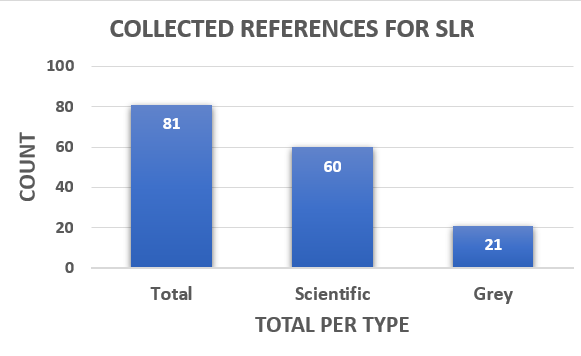
\includegraphics[width=0.5\linewidth]{images/stats_total}	
%	\caption{Total number of collected references used in our systematic literature review (SLR).}
%	\label{fig:stats-total}
%\end{figure}		



\subsection{Data Extraction}

%The data extraction procedure involved reading the full papers and tabulating them in a spreadsheet, and understanding how each study addresses each research question. Data was validated among the peers to discuss the results. A Keen conscientious understanding to identify, analyze and report patterns within the included studies were investigated. Followed the guidelines discussed in \cite{Kitchenham2007} for such studies to explore the introduction and methodology. An integrative approach was applied to categorize the findings. The initial list of categories was derived from the research questions. Data were extracted from a total of 471 included primary studies. A total of 60 publications are finalized and studied. 

For the data extraction procedure, we read all the 81 papers that we collected. For each paper, we focused on understanding and cataloging information that would address our research questions. We categorized the extracted information and stored it on a spreadsheet for easy access. 

More specifically, the data extraction scheme had three main constituents. First, we extracted data about general information of the publication. Second, we extracted data for RQ\#1 and then for RQ\#2. Data for RQ\#1 is specifically related to all the challenges in adopting microservices. Data extracted for RQ\#2 is about the technologies which are used in implementing the microservices and solutions to the challenges are explained in the discussion (Section~\ref{sec:discussion}).
%
By the end of the extraction process, we identified \challengecount distinct categories related to challenges (i.e., RQ\#1), and \techcount different technologies which we grouped into \techgroupcount major categories (i.e., RQ\#2). 
%Our spreadsheet containing the full extracted data is publicly available on our website.\footnote{\url{https://uantwerpen-my.sharepoint.com/:x:/r/personal/s0160228_ad_ua_ac_be/_layouts/15/Doc.aspx?sourcedoc=%7BAA565D3C-022C-4E29-A968-180B213934BA%7D&file=Data_collection.xlsx&action=default&mobileredirect=true}} 

%\henrique{We need to double check the results here, making it sure is is always consistent with the results and the spreadsheet.}

\subsection{Data Synthesis}

%\par The outcomes of the data extractions are discussed in the Result and Discussion section to elaborate their importance regarding research. For the synthesis, two separate spreadsheets were used. 1. Out of the 60 publications, challenges are grouped accordingly and added to a new spreadsheet. 2. The technology/solutions in implementing the microservices and for solving the challenges are added to another spreadsheet. Supporting grey literature to a challenge and a solution was also grouped under the necessary spreadsheets.

For the synthesis, we grouped the categories we extracted from the data extraction into another spreadsheet. That way, we have condensed information where the challenges and technologies/solutions are the main protagonist. For instance, by using this spreadsheet, we can easily find which papers presented a particular challenge. 
%
%We present the outcomes and findings of the synthesized data in Section~\ref{sec:results}.


